\section{Bandwidth Balancing}
In Section~\ref{threshold}, we showed that using a static threshold-based page migration policy alone could
not ideally balance migrating enough pages to maximize GDDR bandwidth utilization while selectively moving
only the hottest data.  In Section~\ref{rangeexpansion}, we showed that informed page prefetching using
a low threshold and range expansion to exploit locality within an application's virtual address space matches or exceeds the performance of a simple threshold-based policy.  Combining low threshold migration with aggressive prefetching drastically
reduces the number of TLB shootdowns at the GPU, reducing the performance overheads of
page migration.  These policies implemented together, however, will continue migrating pages
indefinitely from their initial locations within DDR memory towards the GPU-attached GDDR memory.

\begin{figure}[t]
\centering
    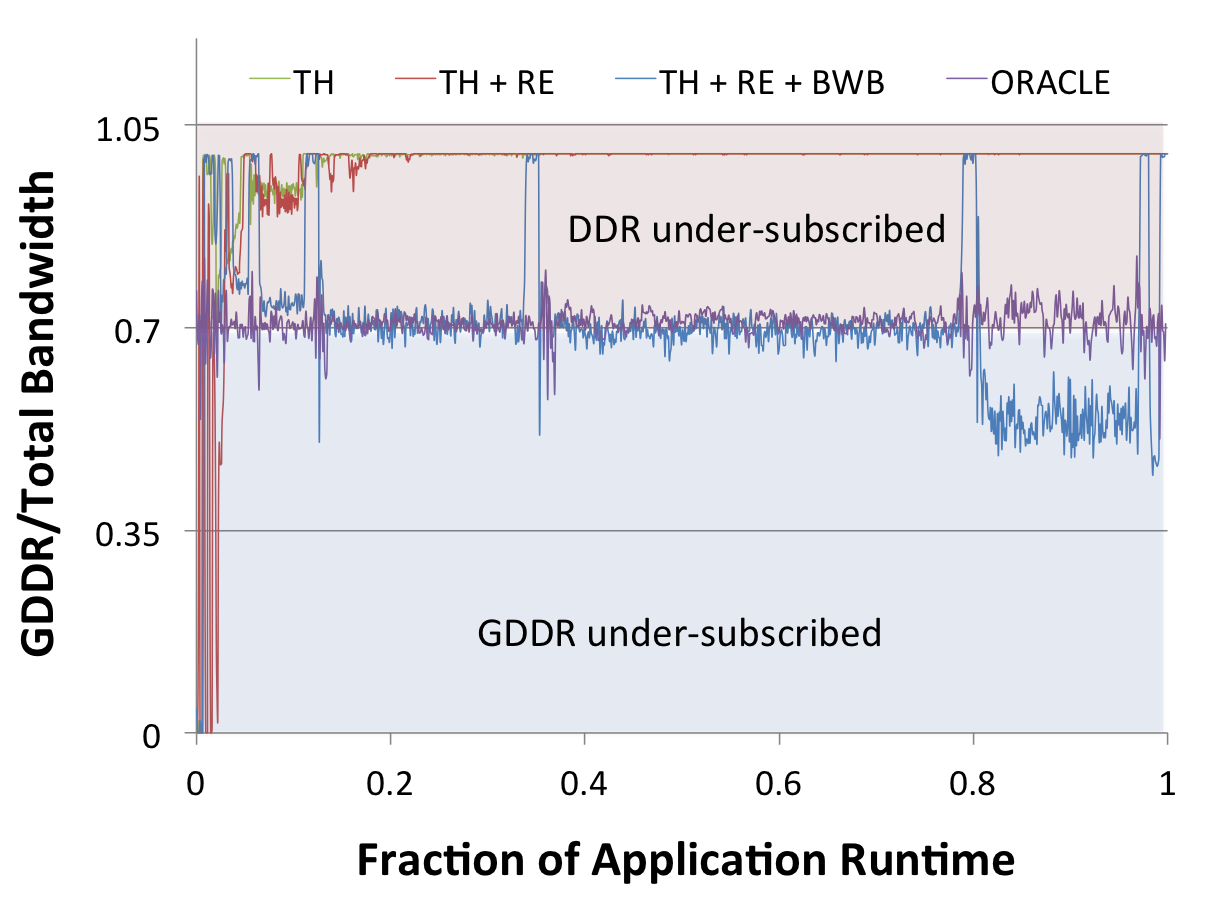
\includegraphics[width=0.9\columnwidth]{hpca2015/figures/bfs-bw-ratio.png}
%    \subfloat[xsbench]{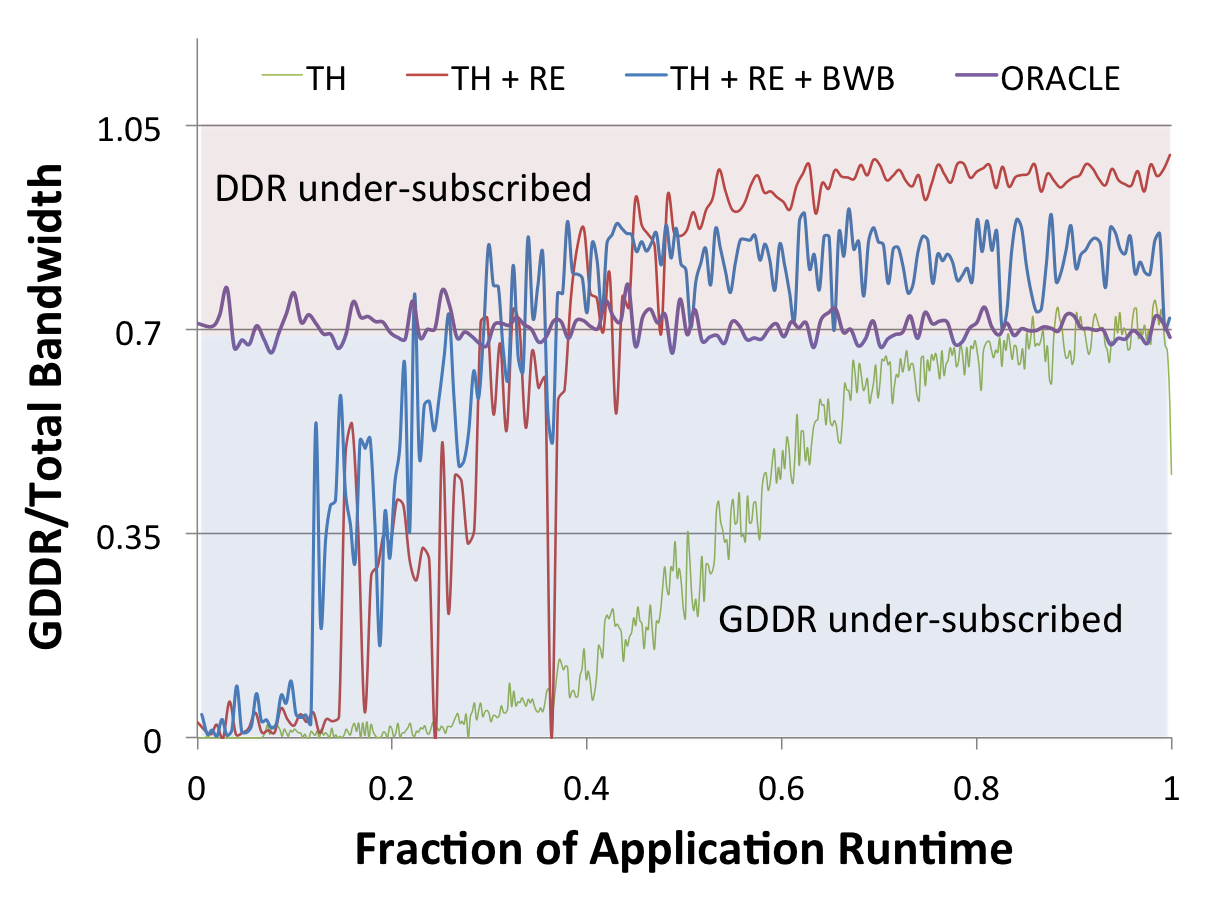
\includegraphics[width=\columnwidth]{hpca2015/figures/xsbench-bw-ratio.png}}\\
%    \subfloat[needle]{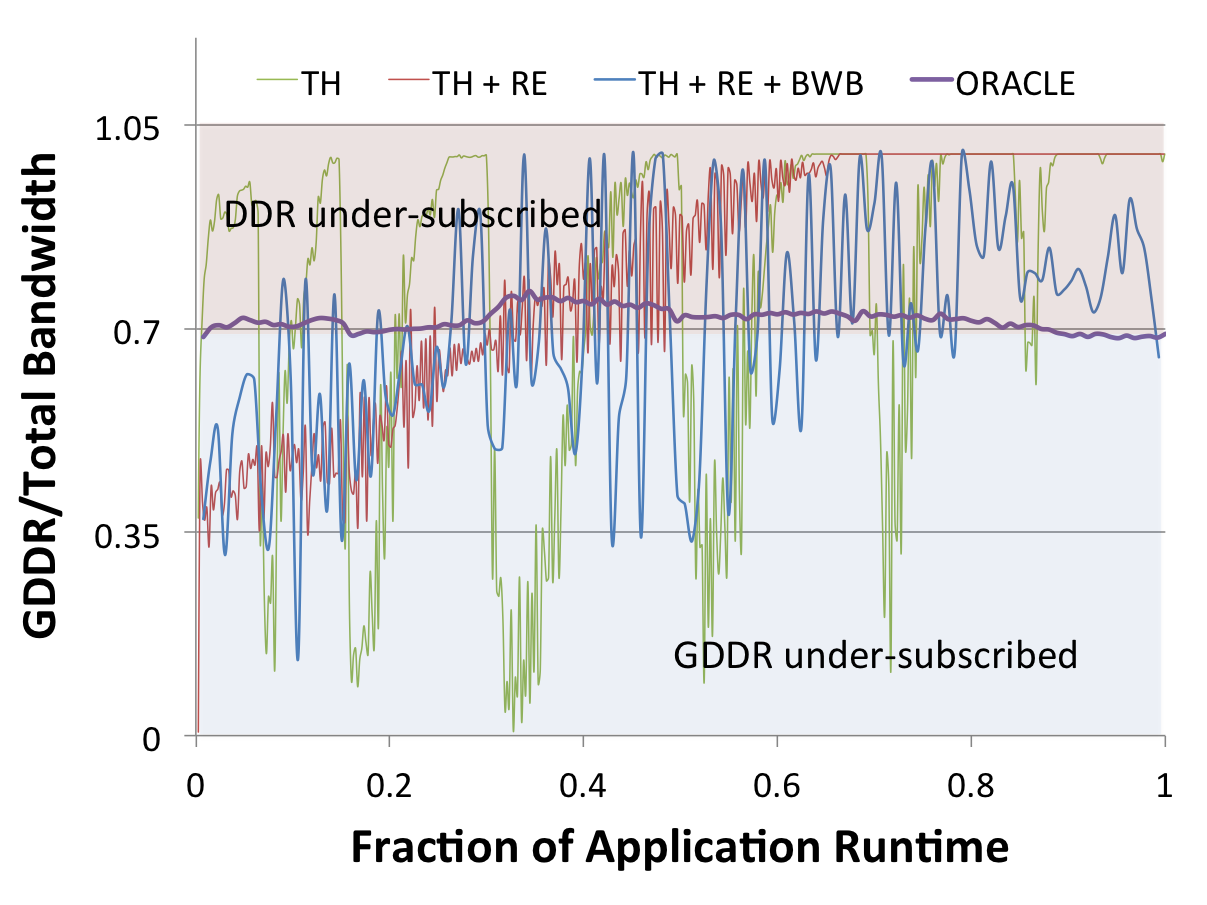
\includegraphics[width=\columnwidth]{hpca2015/figures/needle-bw-ratio.png}}\\
    \caption{{\tt bfs}: Fraction of total bandwidth serviced by GDDR during application
runtime when when using thresholding alone (TH), then adding range expansion
(TH+RE) and bandwidth aware migration (TH+RE+BWB).}
    \label{fig:migrationlimiting-bfs}
\end{figure}

As shown in Figure~\ref{fig:threshold}, however, rather than migrating all pages into the GPU memory,
optimal memory bandwidth utilization is achieved by migrating enough pages to GDDR to maximize its bandwidth while
simultaneously exploiting the additional CPU DDR bandwidth via the hardware cache coherence mechanism.  To prevent
migrating too many pages to GDDR and over-shooting the optimal bandwidth target (70\% of
traffic to GDDR and 30\% to DDR for our system configuration), we implement a migration rate control
mechanism for bandwidth balancing.  Bandwidth balancing, put simply, allows aggressive migration while
the bandwidth ratio of GDDR to total memory bandwidth use is low, and rate limits (or eliminates) migration
as this ratio approaches the system's optimal ratio.
We implement a simple bandwidth balancing policy based on a sampled moving average of the
application's bandwidth needs to each memory type.  We assume that the ideal bandwidth ratio in the system can be known either
via runtime discovery of the system bandwidth capabilities (using an application like stream~\cite{stream_benchmark})
or through ACPI bandwidth information tables, much like memory latency information can be discovered today.

\begin{figure}[t]
\centering
%    \subfloat[bfs]{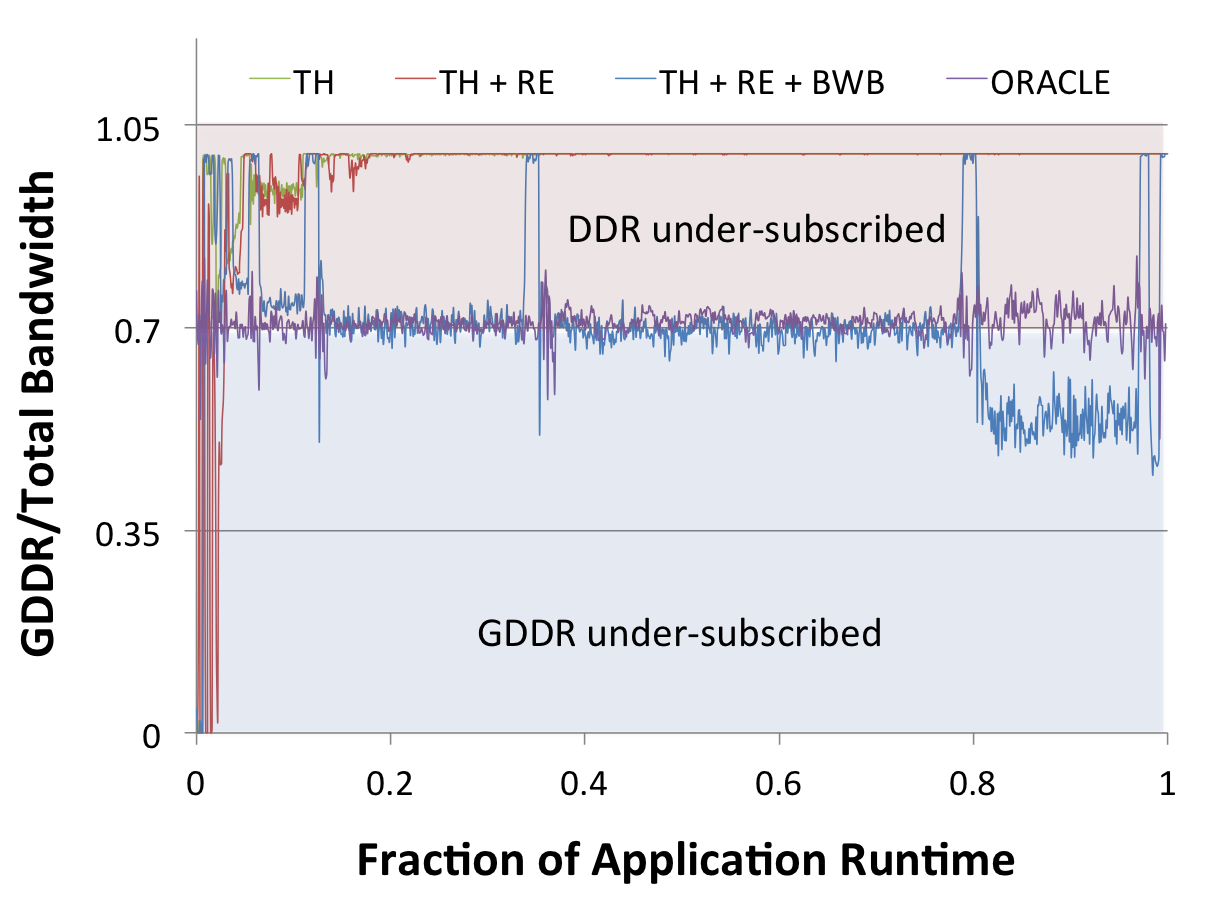
\includegraphics[width=\columnwidth]{hpca2015/figures/bfs-bw-ratio.png}}\\
    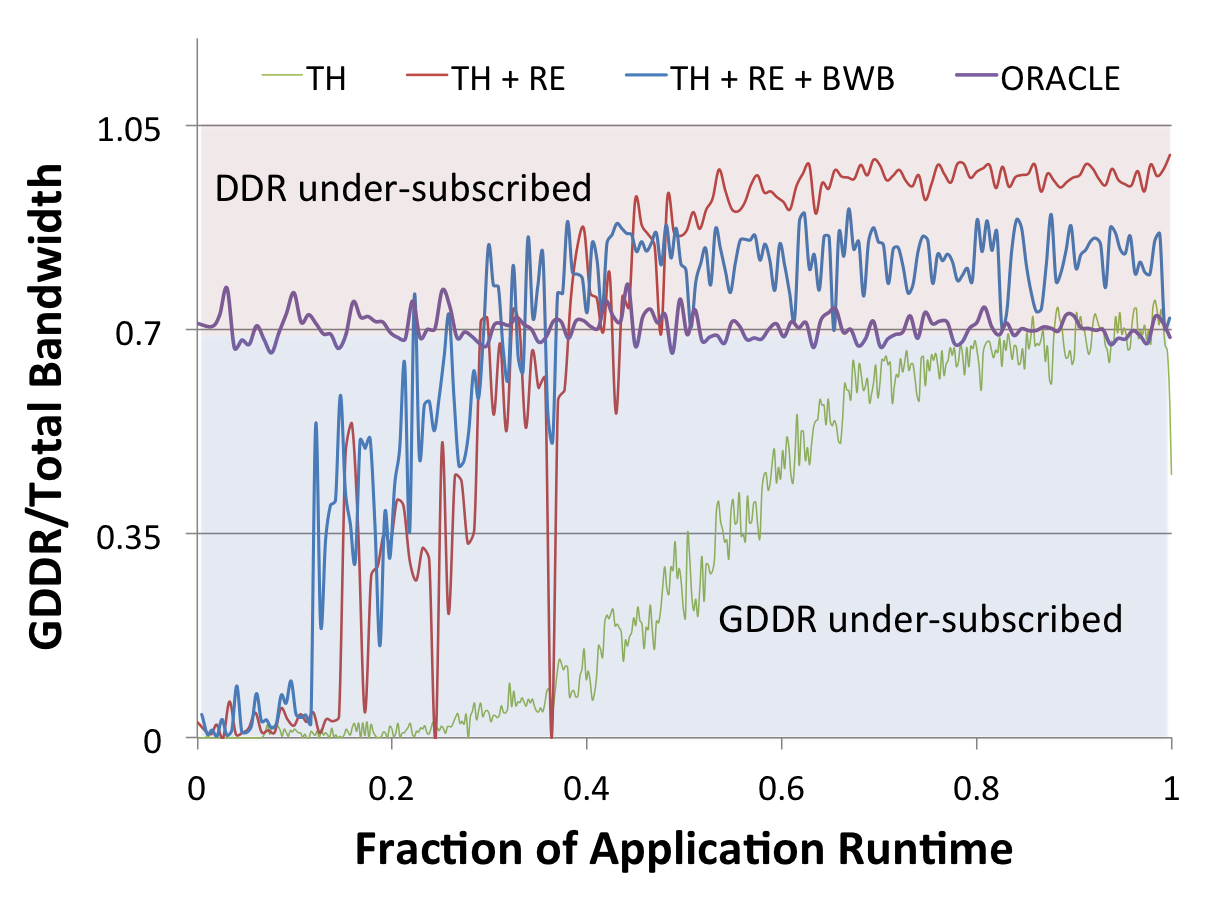
\includegraphics[width=0.9\columnwidth]{hpca2015/figures/xsbench-bw-ratio.png}
%    \subfloat[needle]{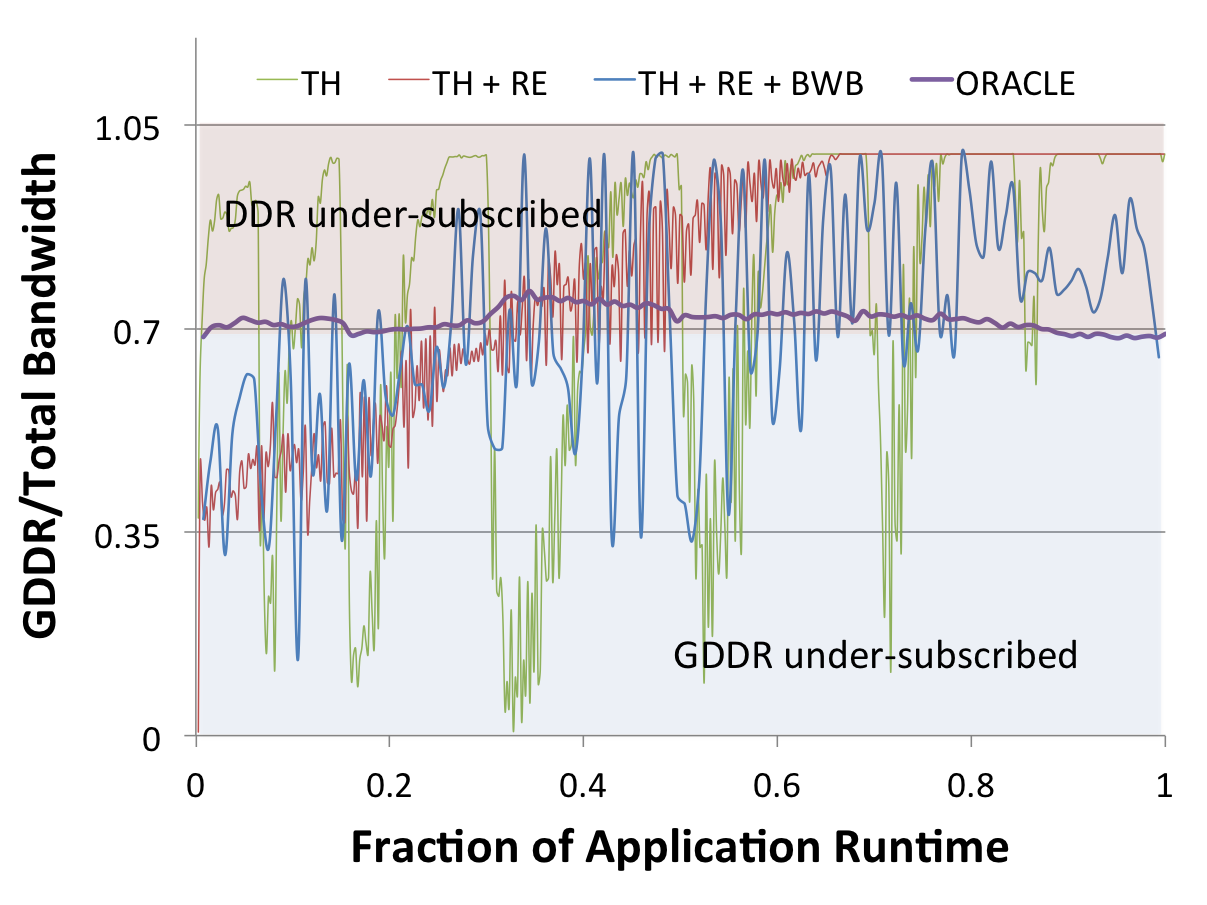
\includegraphics[width=\columnwidth]{hpca2015/figures/needle-bw-ratio.png}}\\
    \caption{{\tt xsbench}: Fraction of total bandwidth serviced by GDDR during application
runtime when when using thresholding alone (TH), then adding range expansion
(TH+RE) and bandwidth aware migration (TH+RE+BWB).}
    \label{fig:migrationlimiting-xsbench}
\end{figure}

\begin{figure}[t]
\centering
%    \subfloat[bfs]{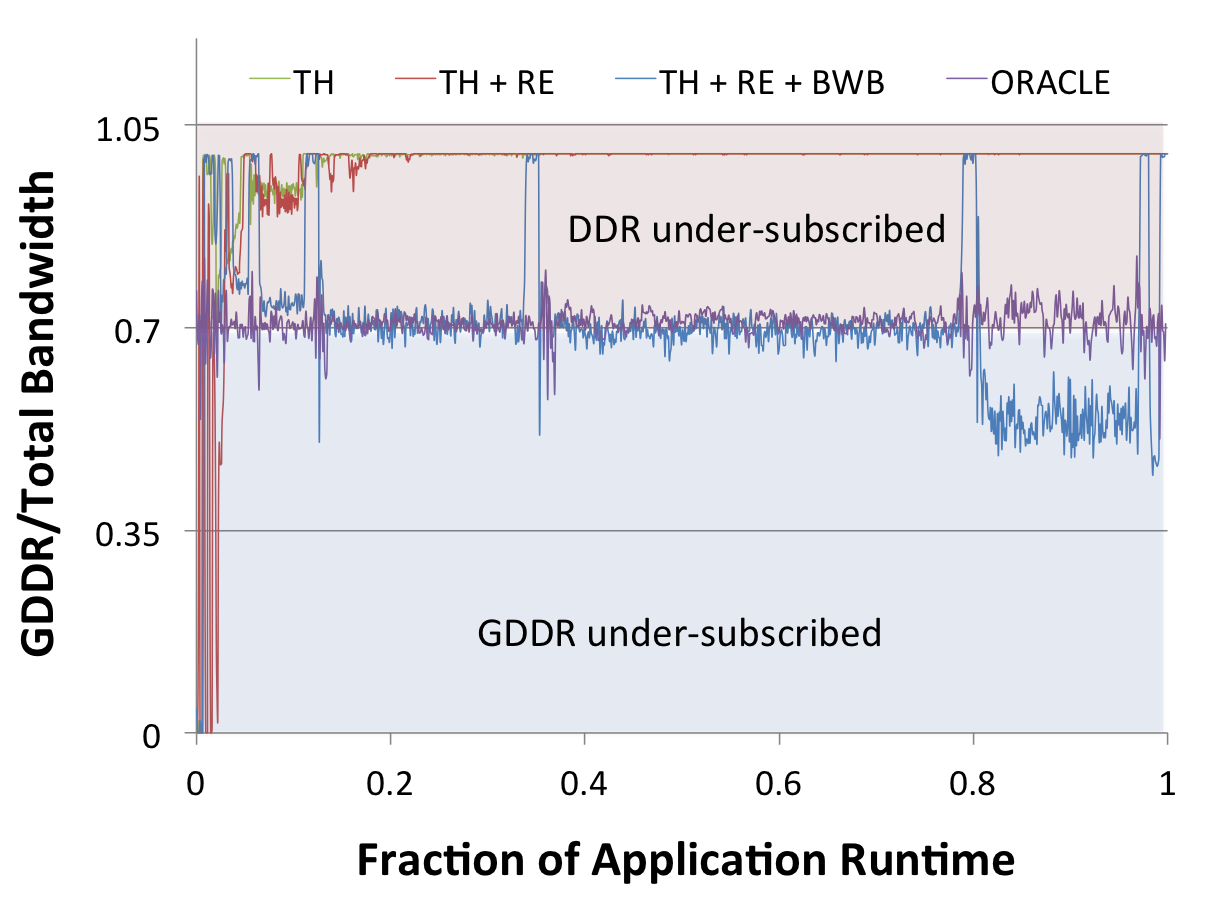
\includegraphics[width=\columnwidth]{hpca2015/figures/bfs-bw-ratio.png}}\\
%    \subfloat[xsbench]{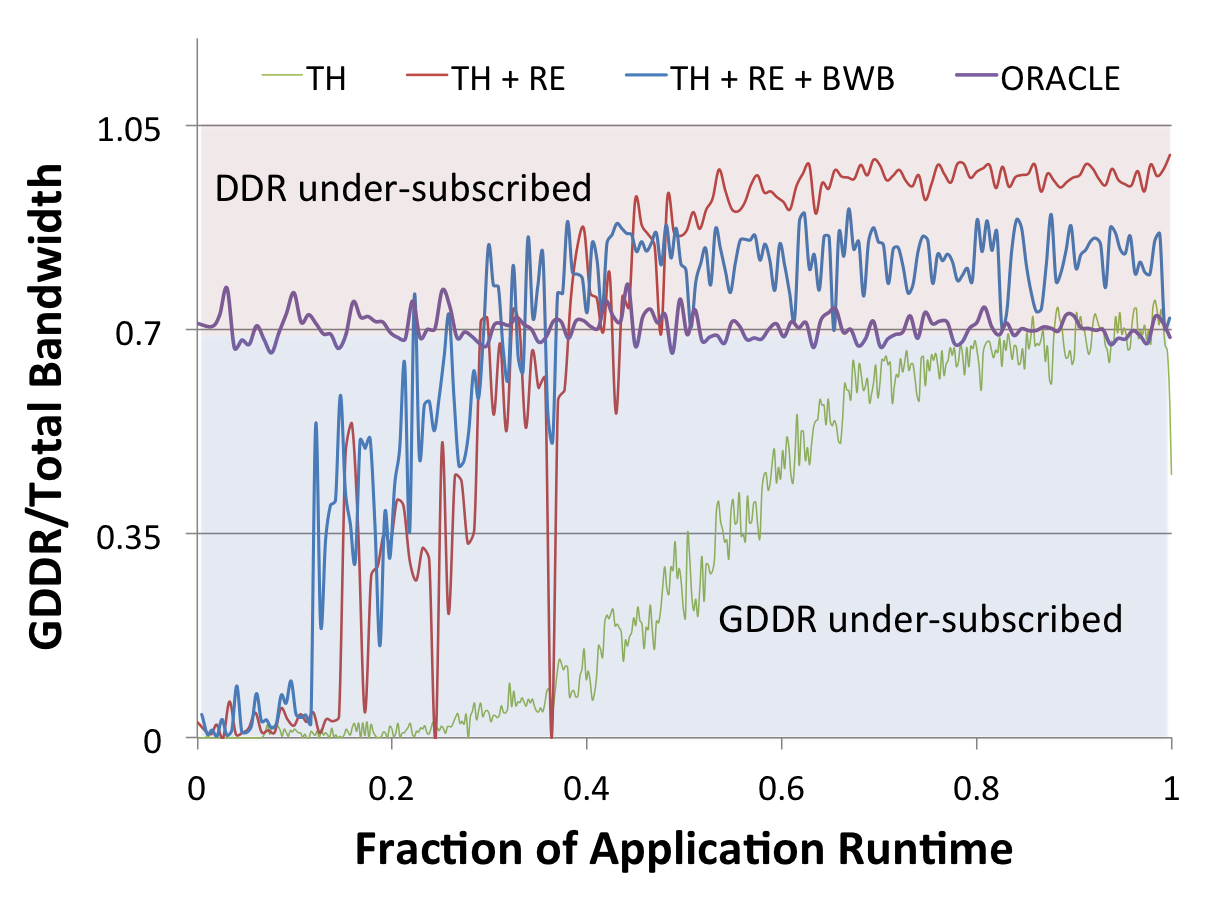
\includegraphics[width=\columnwidth]{hpca2015/figures/xsbench-bw-ratio.png}}\\
    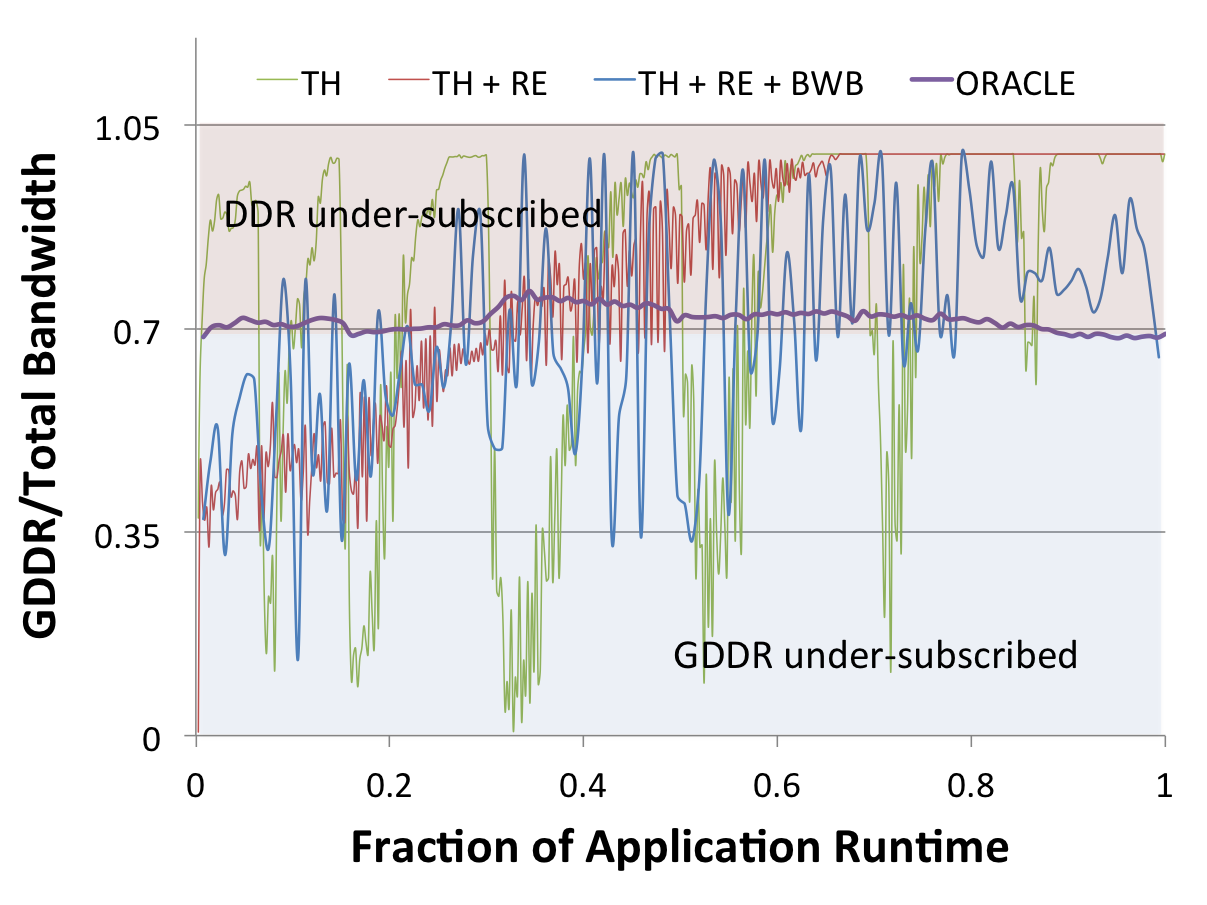
\includegraphics[width=0.9\columnwidth]{hpca2015/figures/needle-bw-ratio.png}
    \caption{{\tt needle}: Fraction of total bandwidth serviced by GDDR during application
runtime when when using thresholding alone (TH), then adding range expansion
(TH+RE) and bandwidth aware migration (TH+RE+BWB).}
    \label{fig:migrationlimiting-needle}
\end{figure}

Given the bandwidth capability of each interface, we can calculate the ideal
fractional ratio, $GDDR / (DDR + GDDR)$, of traffic that should target GDDR
using the methodology defined by Agarwal et al.~\cite{ref:agarwal:asplos2015}.  For the
configuration described in Table~\ref{tab:asplos2015:bw-methodology}, this fraction is
71.4\%.  We currently ignore command overhead variance between the memory
interfaces and assume that it is either the same for technologies in use or that
the optimal bandwidth ratio discovered or presented by ACPI will have taken that
into account.  Using this target, our software page migration samples a
bandwidth accumulator present for all memory channels every 10,000 GPU cycles
and calculates the average bandwidth utilization of the GDDR and DDR in the
system.  If this utilization is below the ideal threshold minus 5\% we continue
migrating pages at full-rate.  If the measured ratio approaches within 5\% of
the target we reduce the rate of page migrations by 1/2.  If the measured ratio
exceeds the target, we suspend further migrations.

\begin{figure*}[thp]
    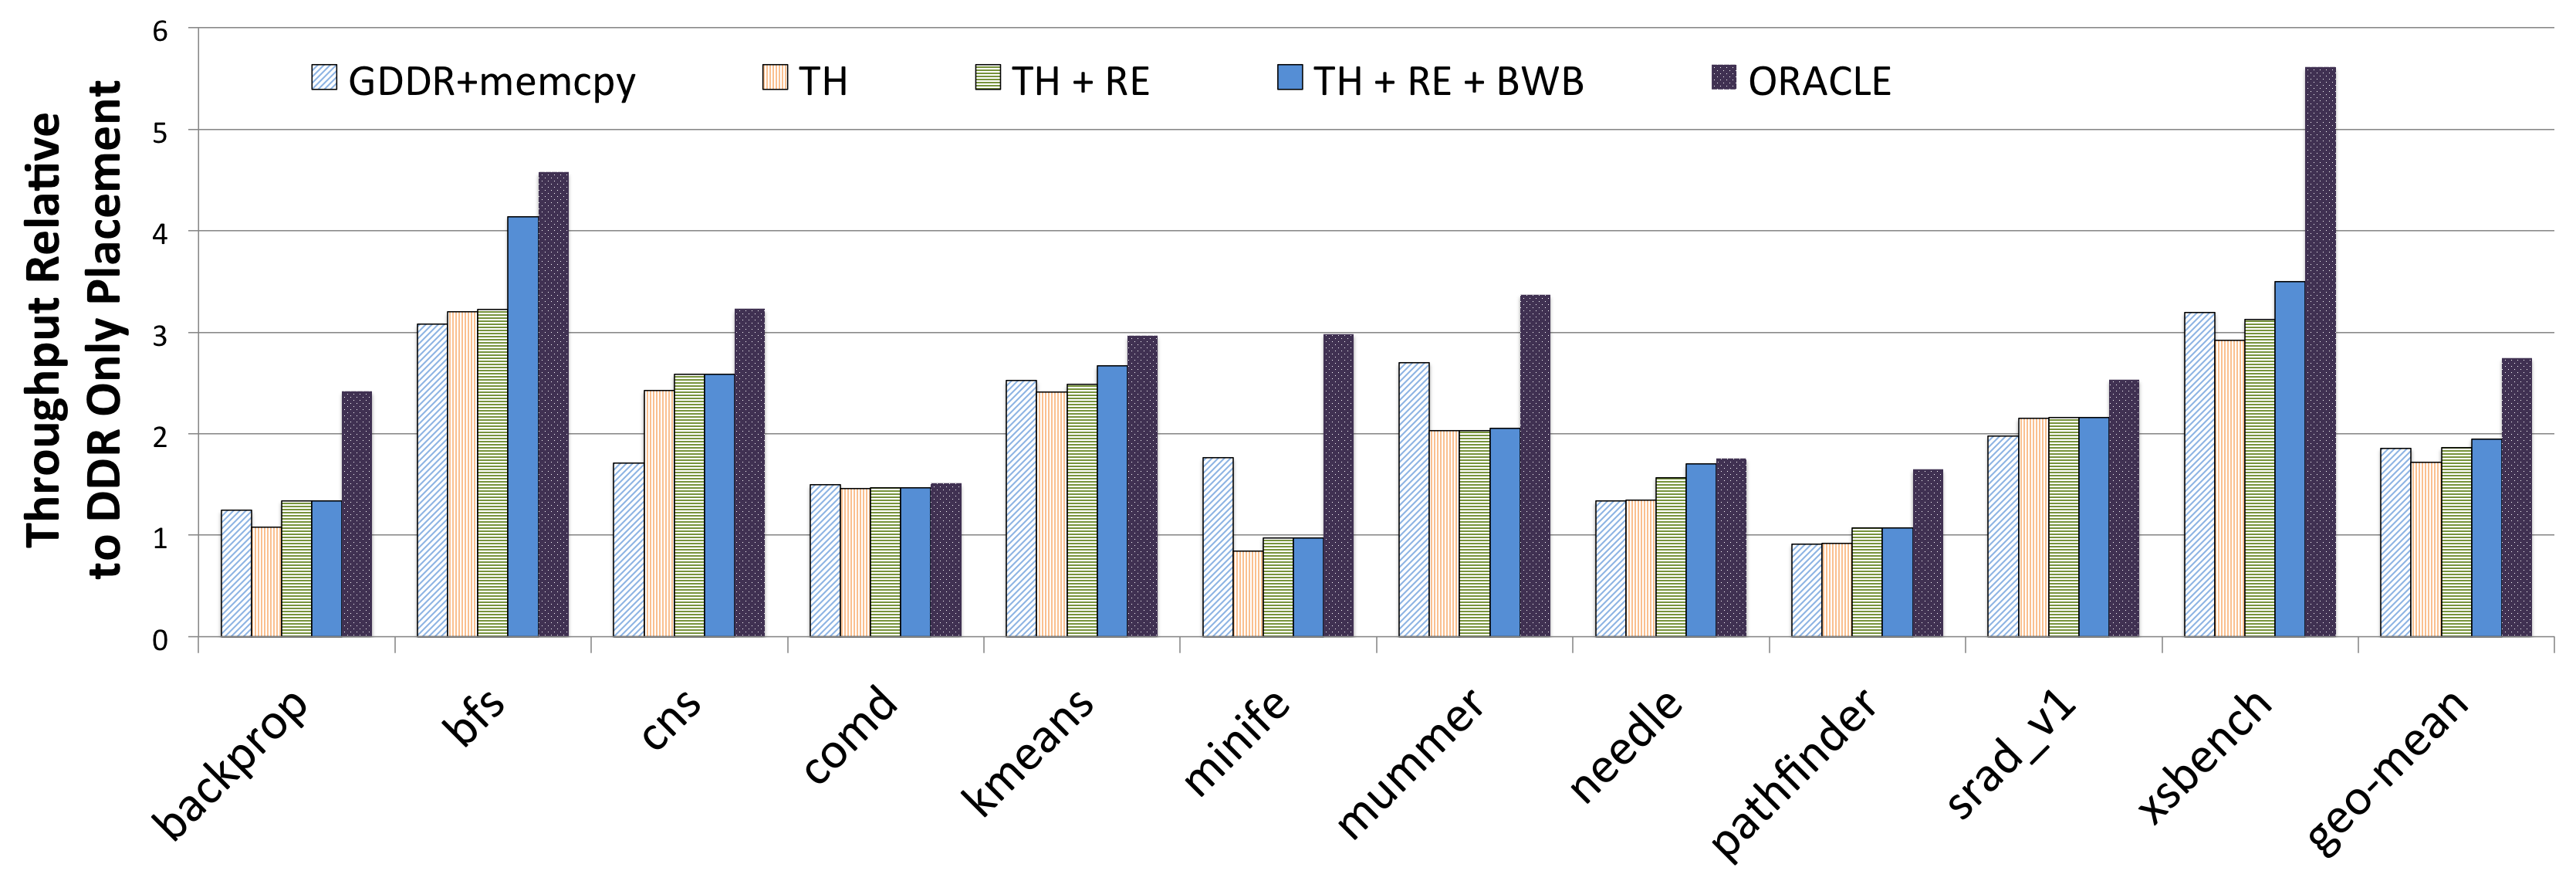
\includegraphics[width=\textwidth]{hpca2015/figures/final.png}
    \caption{Application performance when using thresholding alone (TH), thresholding with range expansion (TH+RE), and thresholding combined with range expansion and bandwidth aware migration (TH+RE+BWB).}
    \label{fig:final}
\end{figure*}

\subsection{Results}
For three example applications,
Figure~\ref{fig:migrationlimiting-bfs},~\ref{fig:migrationlimiting-xsbench},~\ref{fig:migrationlimiting-needle}
shows the bandwidth utilization of the GDDR versus total bandwidth of the application sampled over time
in 1\% increments.  The $TH$ series provides a view of how migration using single page
migration with a static threshold of one (first touch) performs, while $TH+RE$ shows the static threshold with the range expansion
solution described in Section~\ref{rangeexpansion}, and $TH+RE+BWB$ shows this policy with the addition of our
bandwidth balancing algorithm.  The oracle policy shows that if pages were optimally placed \emph{a priori} before execution there would be some,
but not more than 0.1\% variance in the GDDR bandwidth utilization of these applications.  It is also clear that
bandwidth balancing prevents grossly overshooting the targeted bandwidth ratio, as would happen when using thresholds and range expansion alone.

We investigated various sampling periods shorter and longer than 10,000 cycles, but
found that a moderately short window did not cause unwanted migration throttling during the initial
migration phase but facilitated a quick adjustment of the migration policy once the target bandwidth balance was reached.
If an application's bandwidth utilization subsequently dropped below the target, the short window again enabled rapid
reaction to re-enable migration.   While there is certainly room for further refinement (e.g., enabling 
reverse migration when the DDR memory becomes underutilized), our combined solution of threshold-based migration, prefetching via range expansion, and bandwidth balancing is able to capture the majority of the performance available by balancing page migration
with CC-NUMA access.  Figure~\ref{fig:final} shows the results for our implemented solution across
our benchmark suite.  We see that, on average, we are able to not just improve
upon CPU-only DDR by 1.95$\times$,
but also exceed the legacy up-front {\tt memcpy}-based memory transfer paradigm by 6\%,
and achieve 28\% of oracular page placement.

\begin{figure}[bh!]
    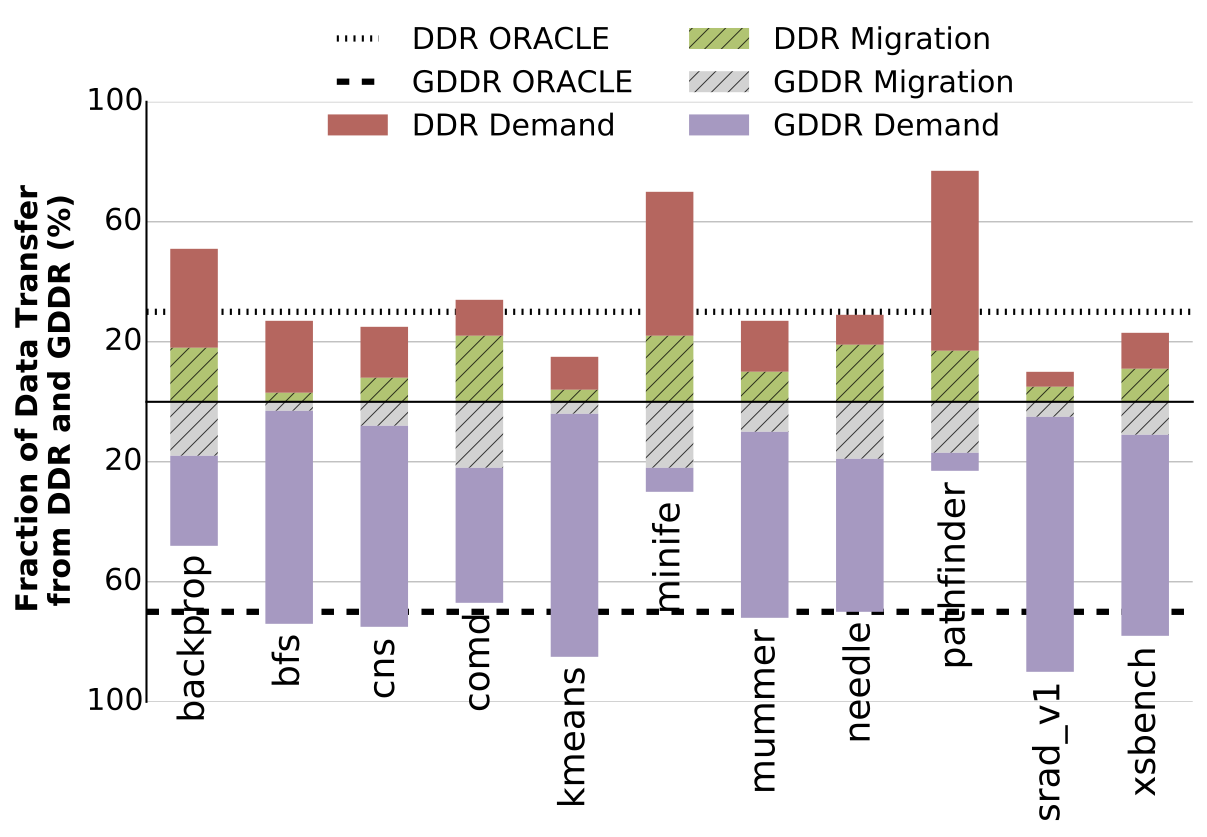
\includegraphics[width=\columnwidth]{hpca2015/figures/bw-util.png}
    \caption{Distribution of memory bandwidth into demand data bandwidth and
migration bandwidth}
    \label{fig:bwutil}
\end{figure}

With our proposed migration policy in place, we seek to understand how it affects the overall bandwidth utilization.  
Figure~\ref{fig:bwutil} shows the fraction of total application bandwidth consumed, divided
into four categories.  The first, DDR Demand is the actual program bandwidth utilization that occurred via CC-NUMA
access to the DDR.  The second and third, DDR Migration and GDDR Migration, are the additional bandwidth overheads on
both the DDR and GDDR that would not have occurred without page migration.  This bandwidth is symmetric because for every read from DDR there is a corresponding write to the GDDR.  Finally, GDDR Demand is the application
bandwidth serviced from the GDDR.  The two additional lines, DDR Oracle and GDDR Oracle, represent
the ideal fractional bandwidth that could be serviced from each of our two memories.

We observe that applications which have the lowest GDDR Demand bandwidth see the least absolute performance improvement from
page migration.  For applications like {\tt minife} and {\tt pathfinder} the GDDR Migration bandwidth also dominates
the GDDR Demand bandwidth utilized by the application. This supports our
conclusion in subsection~\ref{thresholdresults} that migrations may be occurring too late and our mechanisms are not
prefetching the data necessary to make best use of GDDR bandwidth via page migration.  For applications that do perform well 
with page migration, those that perform best tend to have a small amount of GDDR Migration bandwidth when compared to GDDR Demand bandwidth.
For these applications, initial aggressive page migration quickly arrives at the optimal bandwidth balance where our
bandwidth balancing policy then curtails further page migration, delivering good GDDR Demand bandwidth without large migration
bandwidth overhead.
